\chapter{Aproximación}
\section{Motivación}
\noindent
El objetivo de esta sección es el de, dada una función $f(x)$, aproximarla mediante otra función de forma
que minimicemos el área que forman las gráficas de ambas funciones. Para evitar el realizar integrales con
valores absolutos, lo sustituiremos por elevar el área al cuadrado.\\

\noindent
\textbf{Problema de aproximación.} Dados $N$ puntos $\{(x_0, y_0), (x_1, y_1), \ldots, (n_N, y_N)\}$, el problema de aproximar
(ajustar) dichos puntos consiste en encontrar una función $g(x)$, con unas ciertas condiciones, que esté lo más cerca posible
de los puntos.\newline
Esto es, se busca una función $g(x)$ que minimice la distancia a los puntos $(x_i,y_i)~~i=0,1,\ldots, N$.\\

\noindent
Al igual que pasaba con la interpolación, buscamos funciones $g(x)$ que posean propiedades deseables:
\begin{itemize}
    \item Fáciles de implementar.
    \item Fáciles de evaluar.
    \item Simples de calcular.
    \item Suficientemente regulares.
    \item \ldots
\end{itemize}

\noindent
En los siguientes apartados formalizaremos los conceptos de distancia y aproximación.

\section{Producto escalar}
\begin{definicion}[Producto escalar]
    Sea $V$ un espacio vectorial, definimos un producto escalar (o forma bilineal simétrica definida positiva)
    como una aplicación:
    $$\begin{array}{ccccc}
            \langle\cdot,\cdot\rangle & : & V \times V & \longrightarrow & \R                  \\
                                      &   & (u,v)      & \longmapsto     & \langle u,v \rangle
        \end{array}$$

    \noindent
    Que cumple las siguientes propiedades:
    \begin{enumerate}
        \item $\langle v,v\rangle \geq 0~~~~\forall v \in V$
        \item $\langle v,w\rangle = \langle w,v\rangle~~~~\forall v,w \in V$
        \item $\langle \alpha v + \beta w, z\rangle = \alpha \langle v,z\rangle + \beta \langle w,z \rangle~~~~\forall \alpha, \beta \in \R, v,w,z \in V$
        \item $\langle v,v\rangle = 0 \Leftrightarrow v=0 \  \forall v \in V$
    \end{enumerate}

    \noindent
    A un espacio con un producto escalar, $(V, \langle\cdot,\cdot\rangle)$ se le denomina \textbf{espacio con producto escalar}.
\end{definicion}


\begin{ejemplo}Es fácil ver que los siguientes son productos escalares:
\begin{enumerate}
    \item Producto escalar en $\R^n$:

    Sean $u = (u_1, u_2, \ldots, u_n), v=(v_1, v_2, \ldots, v_n) \in V$

    Definimos $\langle u,v\rangle = u_1 v_1 + u_2 v_2 + \ldots + u_n v_n$

    \item Sea $[a,b] \subset \R$ con $a \neq b$, $V=\mathcal{C}([a,b])$ el espacio vectorial de las funciones continuas en $[a,b]$.
    Definimos $\forall f,g \in V$:
    $$\langle f,g\rangle = \int_a^b f(x)g(x)~dx$$

    \item Sea $V=\mathcal{C}([a,b])$, tratamos de definir un producto escalar de la siguiente forma:
    Sean $x_i \in [a,b]~~\forall i \in \{1, \ldots, N\}$. Definimos $\forall f,g \in V$:
    $$\langle f,g\rangle = \sum_{i=1}^N f(x_i)g(x_i)$$
    
    \noindent
    Nos centraremos en comprobar si este producto escalar es válido para un espacio de polinomios.\newline
    Notemos que $\langle f,f \rangle = 0 \Leftrightarrow \sum\limits_{i=1}^N f(x_i)f(x_i)=0 \Leftrightarrow x_i$ es raíz de $f$
    $\forall i \in \{1, \ldots, N\}$\\
    
    \noindent
    Por lo que en $\bb{P}_k$ con $k \geq N \Rightarrow$ podemos tener:
    $$f(x) = \prod_{i=1}^N(x-x_i)$$
    Con $f\neq0 \ \land \ \langle f,f \rangle = 0$, que no define un producto escalar.\\
    
    \noindent
    Sin embargo, en los espacios $\bb{P}_k$ con $k < N$, nuestra aplicación sí define un producto escalar, ya que:
    $$\langle f,f \rangle = 0 \Leftrightarrow \sum_{i=1}^N (f(x_i))^2 = 0 \Leftrightarrow f=0$$
    (Es rutinario comprobar que el producto escalar así definido verifica además las propiedades 1), 2) y 3), por lo que se deja
    al lector a modo de ejercicio su demostración).
\end{enumerate}
\end{ejemplo}

\bigskip
\section{Norma}
\begin{definicion}[Norma]
    Una norma es una aplicación:
    $$\begin{array}{ccccc}
            \|\cdot\| & : & V & \longrightarrow & \R    \\
                      &   & v & \longmapsto     & \|v\|
        \end{array}$$
    Que cumple las siguientes propiedades:
    \begin{enumerate}
        \item $\|v\| \geq 0~~~~\forall v \in V$
        \item $\|v+w\| \leq \|v\|+\|w\|~~~~\forall v,w \in V$
        \item $\|\lambda v\| = |\lambda| \|v\|~~~~\forall \lambda \in \R~~\forall v \in V$
        \item $\|v\|=0 \Leftrightarrow v=0$
    \end{enumerate}

    \noindent
    Un espacio vectorial en el que hay definida una norma se denomina \textbf{espacio vectorial normado}.
\end{definicion}

\begin{teo}[Desigualdad de Cauchy-Schwarz]
    Sea $(V, \langle \cdot , \cdot \rangle)$ un espacio con producto escalar, se verifica:
    $$|\langle u,v \rangle| \leq \|u\|\|v\|~~~~\forall u,v \in V$$
\end{teo}
\begin{proof}
    Sea $\lambda \in \R$, $\forall u,v \in V \Rightarrow \lambda u + v \in V$.
    $$0 \leq \|\lambda u + v\|^2 = \langle \lambda u + v, \lambda u + v \rangle = \lambda^2 \langle u,u \rangle + 2\lambda
        \langle u,v \rangle + \langle v,v \rangle=$$
    $$= \lambda^2 \|u\|^2 + 2\lambda \langle u,v \rangle + \|v\|^2 \geq 0 ~~\forall \lambda \in \R \Leftrightarrow \Delta \leq 0 $$
    $$\Delta = 4\langle u,v \rangle^2 - 4\|u\|^2 \|v\|^2 \leq 0 \Leftrightarrow \langle u,v \rangle^2 \leq \|u\|^2\|v\|^2 \Leftrightarrow$$
    $$\Leftrightarrow \sqrt{\langle u,v \rangle^2} \leq \sqrt{\|u\|^2\|v\|^2} \Leftrightarrow |\langle u,v \rangle| \leq \|u\|\|v\|$$
\end{proof}

\begin{ejemplo} La aplicación de dicha desigualdad con diferentes productos escalares es:
\begin{enumerate}
    \item Producto escalar en $\R^n$:
$$\forall u=(u_1, \ldots, u_n), v=(v_1, \ldots, v_n) \in V~~~~\langle u,v \rangle^2 \leq \|u\|^2\|v\|^2$$
$$(u_1v_1 + u_2v_2 + \ldots + u_nv_n)^2 \leq (u_1^2 + u_2^2 + \ldots + u_n^2)(v_1^2 + v_2^2 + \ldots + v_n^2)$$

    \item \item Sean $f,g\in \cc{C}([a,b])$. Se define $\langle f,g\rangle = \int_a^b f(x)g(x)dx$.

    La desigualdad se escribiría:
    \begin{equation*}
        \left[\int_a^b f(x)g(x)dx\right]^2 \leq \left[\int_a^b f^2(x)dx\right]\left[\int_a^b g^2(x)dx\right]
    \end{equation*}

Tomando $f=1$:
$$\left[ \int_a^b g(x)~dx \right]^2 \leq \int_a^b 1~dx \int_a^b (g(x))^2~dx = (b-a) \int_a^b (g(x))^2~dx$$
\end{enumerate}
    
\end{ejemplo}

\begin{ejercicio}
    Demostrar la desigualdad triangular desde la desigualdad de Cauchy-Schwarz.
    \begin{multline*}
        ||u+v||^2 = \langle u+v,u+v \rangle = ||u||^2 + ||v||^2 +2\langle u,v\rangle \leq ||u||^2 + ||v||^2 +2|\langle u,v\rangle| {\leq}\\ \stackrel{C-S}{\leq} ||u||^2 + ||v||^2 +2||u||||v|| = (||u|| + ||v||)^2
    \end{multline*}

    Tomando raíces cuadradas, tenemos que:
    \begin{equation*}
        ||u+v|| \leq ||u|| + ||v||
    \end{equation*}
\end{ejercicio}

\begin{teo}[Norma inducida]
    En todo espacio vectorial con producto escalar $(V,\langle \cdot,\cdot \rangle)$, podemos definir una norma como sigue:\newline
    Sea $v \in V$, definimos su norma como:
    $$\|v\| = \sqrt{\langle v, v\rangle} \in \R_0^{+}$$
\end{teo}
\begin{proof}
    Claramente la norma así definida es una aplicación $\|\cdot\|:V \rightarrow~\R$.Veamos que cumple las propiedades
    mencionadas en la definición:
    \begin{enumerate}
        \item $$\|v\| = \sqrt{\langle v,v \rangle} \geq 0~~~~\forall v \in V$$
        \item $$\forall u,v \in V: \|u+v\|^2 = \langle u+v, u+v \rangle = \|u\|^2 + 2\langle u,v \rangle + \|v\|^2 \leq$$

        Luego: $$\|u+v\| \leq \|u\|+\|v\|$$
        \item $\forall \lambda \in \R$,$\forall v \in V$:
    $$\|\lambda v\| = \sqrt{\langle \lambda v,\lambda v \rangle} = \sqrt{\lambda^2 \langle v,v \rangle} = |\lambda| \sqrt{\langle v,v \rangle}
        = |\lambda| \|v\|$$

        \item $$\|v\| = 0 \Leftrightarrow \sqrt{\langle v,v \rangle} = 0 \Leftrightarrow \langle v,v \rangle = 0 \Leftrightarrow v=0$$
    \end{enumerate}
\end{proof}

\section{Distancia}
\begin{definicion}[Distancia]
    Una distancia es una aplicación:
    $$\begin{array}{ccccc}
            d & : & V \times V & \longrightarrow & \R     \\
              &   & (u,v)      & \longmapsto     & d(u,v)
        \end{array}$$
    Que cumple las siguientes propiedades:
    \begin{enumerate}
        \item $d(u,v) \geq 0~~~~\forall u,v \in V$
        \item $d(u,v) = d(v,u)~~~~\forall u,v \in V$
        \item $d(u,v) \leq d(u,w) + d(w,v)~~~~\forall u,v,w \in V$
        \item $d(u,v)=0 \Leftrightarrow u=v$
    \end{enumerate}
    
    \noindent
    Un espacio vectorial en el que hay definida una distancia se denomina \textbf{espacio vectorial métrico}.
\end{definicion}

\begin{teo}[Distancia inducida]
    Sea $(V,\langle \cdot,\cdot \rangle)$ un espcio vectorial con producto escalar, podemos definir una distancia como sigue:
    $$d(u,v) = \|u-v\| = \sqrt{\langle u-v,u-v \rangle}~~~~\forall u,v \in V$$
    Aplicando este teorema y el anterior deducimos que todo espacio vectorial con producto escalar $(V,\langle \cdot, \cdot \rangle)$
    es normado y, por tanto, métrico.
\end{teo}
\begin{proof}
    Claramente la distancia así definida es una aplicación $d:V\times V \rightarrow~\R$. Veamos que cumple las propiedades mencionadas en la definición:
    \begin{enumerate}
        \item $$d(u,v) = \|u-v\| \geq 0~~~~\forall u,v \in V$$
        \item $$d(u,v) = \|u-v\| = |-1| \|u-v\| = \|v-u\| = d(v,u)~~~~\forall u,v \in V$$
        \item \begin{multline*}
            d(u,v) = \|u-v\| = \|u-w+w-v\| \leq \|u-w\| + \|w-v\| = d(u,w) + d(w,v)\\\forall u,v,w \in V
        \end{multline*}
    \item $$d(u,v)=0 \Leftrightarrow \|u-v\| = 0 \Leftrightarrow u-v=0 \Leftrightarrow u=v$$
    \end{enumerate}
\end{proof}

\section{Mejor aproximación}
\begin{definicion}[Mejor aproximación]
    Sea $(V, \langle \cdot, \cdot \rangle)$ y $U \subset V$ un subconjunto de $V$.
    Sea $f \in V$. Se dice que $u\in U$ es una mejor aproximación (m.a.) de $f$ en $U$ sii:
    $$d(f,u) =: d(f,U) = \|f-u\| = \inf\{d(f,v) \mid v \in U\}$$
\end{definicion}

\bigskip
\noindent
Nos planteamos a continuación las siguientes cuestiones:
\begin{itemize}
    \item ¿Existe siempre la mejor aproximación?\newline
          No, en el caso de un círculo sin la circunferencia, no existe la mejor aproximación a un punto exterior:
          $$U = \{(x_1,x_2)\in \R^2 \mid x_1^2 + x_2^2 < 1\}~~~~f \in V\setminus U$$
    \item ¿Es única la mejor aproximación?\newline
          No, por ejemplo, si consideramos uan circunferencia, la mejor aproximación a su centro es cada uno de los puntos que
          componen la circunferencia y, por tanto, hay infinitas mejores aproximaciones:
          $$U = \{(x_1, x_2)\in \R^2 \mid x_1^2 + x_2^2 = 1 \}~~~~f = (0,0)$$
\end{itemize}

\noindent
Notemos que minimizar el conjunto (Sea $U$ un subconjunto de $V$)
$$\{d(f,v) \mid v \in U\} = \{\sqrt{\langle f-v, f-v \rangle} \mid v \in U\}$$
es equivalente a minimizar el conjunto:
$$\{d(f,v)^2 \mid v \in U\} = \{\langle f-v, f-v \rangle \mid v \in U\}$$

\noindent
Que es más sencillo de tratar ante la ausencia de la raíz. A este problema se le llama \textbf{aproximación por mínimos cuadrados}.

\begin{definicion}[Ortogonalidad]
    Sean $u,v \in V$, se dice que son ortogonales si:
    $$\langle u,v \rangle = 0$$
    Notado: $u \perp v$.
\end{definicion}

\begin{prop}[Teorema de Pitágoras]
    Sean $u,v\in (V,\langle,\rangle)$.
    \begin{equation*}
        \langle u,v\rangle = 0 \Longrightarrow ||u+v||^2 = ||u||^2 + ||v||^2
    \end{equation*}
\end{prop}
\begin{proof}
    Tenemos que:
    \begin{equation*}
        ||u+v||^2 = \langle u+v,u+v \rangle = ||u||^2 + ||v||^2 +2\cancelto{0}{\langle u,v\rangle} = ||u||^2 + ||v||^2
    \end{equation*}
\end{proof}

\begin{teo}[Caracterización de la mejor aproximación]
    Sea $V$ un espacio con producto escalar, y $U$ un subespacio de $V$. Dada $f\in V$, un elemento $u\in U$ es mejor aproximación de $f$ en $U$ si y solo si:
\begin{equation*}
    \langle f-u,w\rangle = 0\qquad \forall w\in V
\end{equation*}
\end{teo}
\begin{proof}
    Procedemos mediante doble implicación:
    \begin{description}
        \item [$\Longleftarrow$)] Para todo $v\in U$, se cumple:
        \begin{multline*}
            ||f-v||^2 = ||(f-u)+(u-v)||^2 = ||f-u||^2 + ||u-v||^2 +2\cancelto{0}{\langle f-u,u-v\rangle} = \\=
            ||f-u||^2 +||u-v||^2 \leq 0 \Longrightarrow ||f-v||^2 \geq ||u-v||^2 \qquad \forall v\in V
        \end{multline*}

        donde he aplicado que $U$ es un sucespacio vectorial, por lo que $u-v\in U$, y por tanto $\langle f-u,u-v\rangle = 0$ por hipótesis.

        Por tanto, tenemos que $||u-v||\leq ||f-v|| \qquad \forall v\in V$, por lo que $u$ es la mejor aproximación en $U$ de $f$.

        \item [$\Longrightarrow$)] Por ser $u$ la mejor aproximación de $f$, tenemos que:
        \begin{equation*}
            ||f-u||\leq ||f-w|| \Longrightarrow ||f-u||^2\leq ||f-w||^2 \qquad \forall w\in U
        \end{equation*}

        Tomamos $v\in U$, y sea $w=u+\lambda v \in U \mid \lambda \in \bb{R}$. Por tanto, como $w\in U$, tenemos que:
        \begin{equation*}
            ||f-u||^2\leq ||f-u-\lambda v||^2 = \langle f-u-\lambda v, f-u-\lambda v\rangle = ||f-u||^2 -2\lambda \langle f-u,v\rangle +\lambda^2 ||v||^2
        \end{equation*}

        Por tanto,
        \begin{equation*}
            0 \leq -2\lambda \langle f-u,v\rangle +\lambda^2 ||v||^2 
            = \lambda (\lambda ||v||^2 -2 \langle f-u,v\rangle) 
            \qquad \forall \lambda\in \bb{R}, \forall v\in U.
        \end{equation*}

        Las raíces de dicha parábola en la incógnita $\lambda \in \bb{R}$ son:
        \begin{equation*}
            \lambda_1 = 0 \qquad \lambda_2 = \frac{2\langle f-u,v\rangle}{||v||^2}
        \end{equation*}

        Por tanto, como es siempre $\geq 0$, tenemos que las dos raíces son iguales. Por tanto, $\langle f-u,v\rangle = 0$.
    \end{description}
\end{proof}


\subsection{Método para el cálculo de la mejor aproximación}
\begin{teo}[existencia y unicidad de la mejor aproximación]
    Sea $(V, \langle \cdot, \cdot \rangle)$ y $U \subseteq V$ subespacio vectorial de $V$ de dimensión finita, entonces la mejor
    aproximación existe y es única.
\end{teo}
\begin{proof}
    Buscamos $u \in U = \cc{L}\{\varphi_0, \varphi_1, \ldots, \varphi_m\} \Rightarrow \exists a_0, a_1, \ldots, a_m \in \R$ tal que:
    $u = a_0 \varphi_0 + a_1 \varphi_1 + \ldots + a_m \varphi_m$. Buscamos calcular $a_i~~\forall i \in \{0, \ldots, m\}$:\\

    \noindent
    Se tiene que $u$ es la mejor aproximación de $f \in V$ en $U$:
    $$\Leftrightarrow \langle f-u, v\rangle = 0~~\forall v \in U \Leftrightarrow \langle f-u, \varphi_k\rangle = 0~~\forall k \in \{0, \ldots, m\} \Leftrightarrow$$
    $$\Leftrightarrow \langle f-u, \varphi_k\rangle = \langle f-(a_0\varphi_0 + a_1\varphi_1 + \ldots + a_m\varphi_m),\varphi_k\rangle = $$
    $$ =\langle f,\varphi_k \rangle -a_0 \langle \varphi_0,\varphi_k \rangle - a_1\langle \varphi_1,\varphi_k \rangle - \ldots - a_m \langle
        \varphi_m,\varphi_k \rangle = 0 \Leftrightarrow$$
    $$\Leftrightarrow a_0 \langle \varphi_0,\varphi_k \rangle + a_1\langle \varphi_1,\varphi_k \rangle + \ldots - a_m \langle
        \varphi_m,\varphi_k \rangle = \langle f,\varphi_k \rangle~~\forall k \in \{0, \ldots, m\}$$
    Que nos da el siguiente sistema de ecuaciones lineales de $m+1$ ecuaciones y $m+1$ incógnitas:
    $$\left( \begin{array}{cccc}
                \langle \varphi_0,\varphi_0 \rangle & \langle \varphi_1,\varphi_0 \rangle & \ldots & \langle \varphi_m,\varphi_0 \rangle \\
                \langle \varphi_0,\varphi_1 \rangle & \langle \varphi_1,\varphi_1 \rangle & \ldots & \langle \varphi_m,\varphi_1 \rangle \\
                \vdots                              & \vdots                              & \ddots & \vdots                              \\
                \langle \varphi_0,\varphi_m \rangle & \langle \varphi_1,\varphi_m \rangle & \ldots & \langle \varphi_m,\varphi_m \rangle
            \end{array} \right) \left( \begin{array}{c}
                a_0    \\
                a_1    \\
                \vdots \\
                a_m
            \end{array} \right) = \left( \begin{array}{c}
                \langle f,\varphi_0 \rangle \\
                \langle f,\varphi_1 \rangle \\
                \vdots                      \\
                \langle f,\varphi_m \rangle
            \end{array} \right)$$
    A la matriz de coeficientes anterior se le llama matriz de Gram y verifica que es simétrica y definida positiva, por lo que
    el sistema anterior es compatible determinado, luego sabemos que los coeficientes $a_i~~i\in\{0, \ldots, m\}$ existen y que
    son únicos.
\end{proof}


\begin{ejemplo}
    Calcular la mejor aproximación de la función $f(x)=x^3$ en $\bb{P}_1$, utilizando el producto escalar definido como:
$$\langle v,u \rangle = \int_{-1}^1v(x)u(x)~dx~~~~\forall u,v \in V$$


\noindent
$\bb{P}_1 = \cc{L}\{1,x\}$, la mejor aproximación de $f$ será $u(x) = a_0 \cdot 1 + a_1x \in \bb{P}_1~~~a_0,a_1 \in \R$
$$\left( \begin{array}{cc}
            \langle 1,1 \rangle & \langle x,1 \rangle \\
            \langle 1,x \rangle & \langle x,x \rangle
        \end{array} \right) \left( \begin{array}{c}
            a_0 \\
            a_1
        \end{array} \right) = \left( \begin{array}{c}
            \langle x^3,1 \rangle \\
            \langle x^3,x \rangle
        \end{array} \right)$$
$$\langle 1,1 \rangle = 2$$
$$\langle 1,x \rangle = \langle x,1 \rangle = 0$$
$$\langle x,x \rangle = \dfrac{2}{3} $$
$$\langle x^3,1 \rangle = 0$$
$$\langle x^3,x \rangle = \dfrac{2}{5}$$

$$\left. \begin{array}{cccc}
        2a_0 &                 & = & 0            \\
             & \dfrac{2}{3}a_1 & = & \dfrac{2}{5}
    \end{array} \right\} \Rightarrow \left\{ \begin{array}{c}
        a_0 = 0 \\
        a_1 = \dfrac{3}{5}
    \end{array} \right\} \Rightarrow u(x) = \dfrac{3}{5}x$$
\end{ejemplo}



\begin{ejemplo}
    Calcular la recta que mejor aproxima por mínimos cuadrados los datos $\{(1,0),(2,1),(3,2),(4,3),(5,4)\}$.
Siendo $U=\cc{L}\{1,x\}$ y el producto escalar en $U$ se define como:
$$\langle v,w \rangle = v(1)w(1) + v(2)w(2) + v(3)w(3) + v(4)w(4) + v(5)w(5)~~~~\forall v,w \in V$$
La mejor aproximación de los puntos será $u(x) = a_0 \cdot 1 + a_1x \in \bb{P}_1~~~a_0,a_1 \in \R$
$$\left( \begin{array}{cc}
            \langle 1,1 \rangle & \langle x,1 \rangle \\
            \langle 1,x \rangle & \langle x,x \rangle
        \end{array} \right) \left( \begin{array}{c}
            a_0 \\
            a_1
        \end{array} \right) = \left( \begin{array}{c}
            \langle f,1 \rangle \\
            \langle f,x \rangle
        \end{array} \right)$$
$$\langle 1,1 \rangle = 5$$
$$\langle 1,x \rangle = \langle x,1 \rangle = 15$$
$$\langle x,x \rangle = 55 $$
$$\langle f,1 \rangle = 10$$
$$\langle f,x \rangle = 40$$

$$\left. \begin{array}{cccc}
        5a_0  & 15a_1 & = & 10 \\
        15a_0 & 55a_1 & = & 40
    \end{array} \right\} \Rightarrow \left\{ \begin{array}{c}
        a_0 = -1 \\
        a_1 = 1
    \end{array} \right\} \Rightarrow u(x) = -1+x$$
\end{ejemplo}



\subsection{Tipos de aproximación por mínimos cuadrados}
\noindent
\subsubsection{Aproximación por mínimos cuadrados continua}

Para la aproximación por mínimos cuadrados continua en el intervalo $[a,b]\subset \bb{R}$ se emplea el producto escalar siguiente:
\begin{equation*}
    \langle f,g\rangle = \int_{a}^b \omega(x)f(x)g(x)dx
\end{equation*}

donde $\omega$ es denominada \emph{función peso} y ha de ser integrable y $\omega\geq 0 \quad \forall x\in [a,b]$. Si no se especifica lo contrario, $\omega(x)=1$.

\begin{ejemplo}
    Sea el producto escalar definido como
    \begin{equation*}
        \langle f,g\rangle = \int_{-1}^1 f(x)g(x)dx
    \end{equation*}

    Encontrar la mejor aproximación de $f(x)=x^3$ en $\bb{P}_1$.

    Sea $u\in \bb{P}_1$ la mejor aproximación de $f$. Tomamos como base $\bb{P}_1=\cc{L}\{1,x\}$, por lo que sea $u(x)=a_0\cdot 1 + a_1x \quad a_0,a_1\in \bb{R}$. El sistema a resolver, por tanto, es:
    \begin{equation*}
        \left\{\begin{array}{c}
            a_0\langle 1,1\rangle + a_1 \langle x,1\rangle = \langle x^3, 1 \rangle \\
            a_0\langle 1,x\rangle + a_1 \langle x,1\rangle = \langle x^3, x \rangle \\
        \end{array}\right.
    \end{equation*}

    Tras calcular cada integral definida, tenemos que:
    \begin{equation*}
        \left\{\begin{array}{c}
            2a_0 + 0\cdot a_1 = 0 \\
            0\cdot a_0 + \frac{2}{3} a_1 = \frac{2}{5}
        \end{array}\right.
    \end{equation*}

    Por tanto, $u(x)=\frac{3}{5}x$.
    \begin{figure}[H]
        \centering
        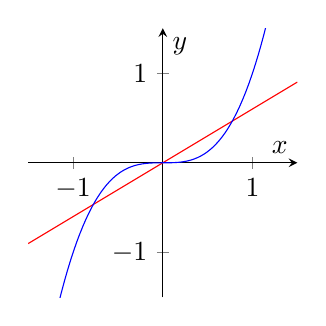
\begin{tikzpicture}
        \begin{axis}[
            xlabel=$x$,
            ylabel=$y$,
            xmin=-1.5,
            xmax=1.5,
            ymin=-1.5,
            ymax=1.5,
            axis lines=middle,
            width=5cm,
            height=5cm,
            samples=90 % número de muestras para la función
        ]
        
        \addplot[red ,domain=-1.5:1.5] {3/5*x};
        \addplot[blue ,domain=-1.5:1.5] {x^3};
            
        \end{axis}
        \end{tikzpicture}
    \end{figure}
\end{ejemplo}


\subsubsection{Aproximación por mínimos cuadrados discreta}
Para la aproximación por mínimos cuadrados discreta en los nodos $x_i\subset \bb{R}$, con $i=0,\dots, N$; se emplea el producto escalar siguiente:
\begin{equation*}
    \langle f,g\rangle = \sum_{i=0}^N \omega(x_i)f(x_i)g(x_i)dx
\end{equation*}

donde $\omega$ es denominada \emph{función peso} y ha de ser $\omega(x_i) > 0 \quad \forall i=0,\dots, N$. Si no se especifica lo contrario, $\omega(x)=1$.

El problema de la mejor aproximación por mínimos cuadrados discreta consiste en lo siguiente:

Sea $f:[a,b]\to \bb{R}$ para la que conocemos $(x_i, f(x_i))\quad i=0,\dots, N$. Encontrar $p\in \bb{P}_m$ donde $m<N$ tal que:
\begin{equation*}
    ||f-p||^2 = \min_{q\in \bb{P}_m} ||f(x)-q(x)||^2 = \lim_{q\in \bb{P}_m} \sum_{k=0}^N [f(x_k)-q(x_k)]^2
\end{equation*}

donde he considerado el producto escalar definido como:
\begin{equation*}
    \langle f,g \rangle = \sum_{k=0}^N f(x_k)g(x_k)
\end{equation*}

Alternativamente, trabajamos de la siguiente manera. Sabemos que $\dim \bb{P}_m = m+1$. Consideramos 
\begin{equation*}
    \bb{P}_m = \cc{L}\{\varphi_0,\dots,\varphi_N\}
\end{equation*}

y la aplicación
\begin{equation*}
    \varphi_k \longmapsto \Phi=\left(\begin{array}{c}
        \varphi_k (x_0) \\ \varphi_k(x_1) \\ \vdots \\ \varphi_k(x_N)
    \end{array}\right)
\end{equation*}


Por la misma aplicación, tenemos que
\begin{equation*}
    f\longmapsto F=\left(\begin{array}{c}
        f(x_0) \\ f(x_1) \\ \vdots \\ f(x_N)
    \end{array}\right)
\end{equation*}


Consideramos $\nu = \cc{L}\{\Phi_0, \Phi_1, \dots, \Phi_m\}$, y demostremos que forman base.
\begin{equation*}
    a_0 \Phi_0 + a_1\Phi_1 + \dots a_m\Phi_m = 0 \Longrightarrow
    a_0\varphi_0(x_k) + \dots + a_m\varphi_m(x_k)=0 \qquad \forall k=0,\dots,N
\end{equation*}

Por tanto, como se anulan para todo $k$, tenemos que:
\begin{equation*}
    a_0\varphi_0 + \dots + a_m\varphi_m = 0 \Longrightarrow a_0=\dots=a_m=0
\end{equation*}

Por tanto, el problema se reduce a encontrar $P$ mejor aproximación de $F$ en $\nu$ con el producto escalar euclídeo.

No obstante, tenemos que:
\begin{equation*}
    \langle \Phi_i, \Phi_j\rangle = \sum_{k=0}^N \varphi_i(x_k)\varphi_j(x_k)
\end{equation*}
por tanto, tenemos que hemos llegado al producto escalar discreto definido en el primer caso.


\begin{ejemplo}
    Calcular la recta que mejor aproxima por mínimos cuadrados los siguientes datos:
    \begin{equation*}
        (1,0) \quad (2,1) \quad (3,2) \quad (4,3) \quad (5,4)
    \end{equation*}

    Sea el producto escalar definidio como:
    \begin{equation*}
        \langle u,v\rangle = \sum_{i=0}^N u(x_i)v(x_i)
    \end{equation*}

    Buscamos aproximar en $U=\bb{P}_1=\cc{L}\{1,x\}$. $f(x)$ está definida por:
    \begin{equation*}
        \left(\begin{array}{c}
            f(1) \\ f(2) \\ f(3) \\ f(4) \\ f(5)
        \end{array}\right)
        = \left(\begin{array}{c}
            0 \\ 1 \\ 2 \\ 3 \\ 4
        \end{array}\right)
    \end{equation*}

    Sea $u \in \bb{P}_1$ la mejor aproximación de $f$. Sea $u=a_0 \cdot 1 + a_1\cdot x$. El sistema a resolver, por tanto, es:
    \begin{equation*}
        \left\{\begin{array}{c}
            a_0\langle 1,1\rangle + a_1 \langle x,1\rangle = \langle f, 1 \rangle \\
            a_0\langle 1,x\rangle + a_1 \langle x,x\rangle = \langle f, x \rangle \\
        \end{array}\right.
    \end{equation*}

    Tenemos que:
    \begin{equation*}
        \begin{array}{c|c|c|c|c|c|c}
            x_i & f_i & x_1^0 & x_i^1 & x_i^2 & x_i^0f_i & x_i^1f_i \\ \hline
            1 & 0 & 1 & 1 & 1 & 0 & 0 \\
            2 & 1 & 1 & 2 & 4 & 1 & 2 \\
            3 & 2 & 1 & 3 & 9 & 2 & 6 \\
            4 & 3 & 1 & 4 & 16 & 3 & 12 \\
            5 & 4 & 1 & 5 & 25 & 4 & 20 \\ \hline
            && 5 & 15 & 55 & 10 & 40 \\
            && (\langle 1,1 \rangle) & (\langle 1,x \rangle) &
            (\langle x,x \rangle) & 
            (\langle f,1 \rangle) &
            (\langle f,x \rangle)
            
        \end{array}
    \end{equation*}

    Calculando cada producto escalar, tenemos que el sistema a resolver es:
    \begin{equation*}
        \left\{\begin{array}{c}
            5a_0 + 15a_1 = 10 \\
            15a_0 + 55a_1 = 40
        \end{array}\right.
    \end{equation*}

    Resolviendo, tenemos que $a_0=-1,\;a_1=1$.

    Por tanto, $u(x)=-1+x$.
\end{ejemplo}

\subsection{Ejemplos de Chebyshev}
\begin{itemize}
    \item \textbf{Ejemplo de Chebyshev de primera especie.}
En este caso, se toma:
$$w(x) = \dfrac{1}{\sqrt{1-x^2}}~~\forall x \in ]-1,1[$$
Esta función da un gran peso a los puntos que se encuentran en los extremos y un peso menor a los puntos centrales.

        \begin{figure}[H]
            \centering
            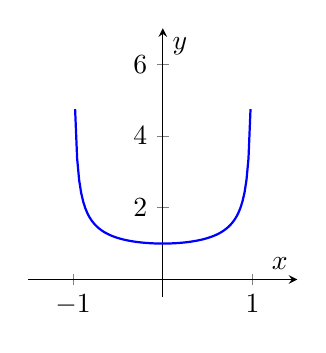
\begin{tikzpicture}
            \begin{axis}[
                xlabel=$x$,
                ylabel=$y$,
                xmin=-1.5,
                xmax=1.5,
                ymin=-0.5,
                ymax=7,
                axis lines=middle,
                width=5cm,
                height=5cm,
                samples=90 % número de muestras para la función
            ]
            
            \addplot[blue, thick, domain=-1:1] {1/sqrt(1-x^2)};
            \end{axis}
            \end{tikzpicture}
        \end{figure}

    \item \textbf{Ejemplo de Chebyshev de segunda especie.}
$$w(x) = \sqrt{1-x^2}~~\forall x \in [-1,1]$$
Esta función da un gran peso a los puntos centrales y un menor peso (casi inapreciable) a los puntos en lo extremos.
        \begin{figure}[H]
            \centering
            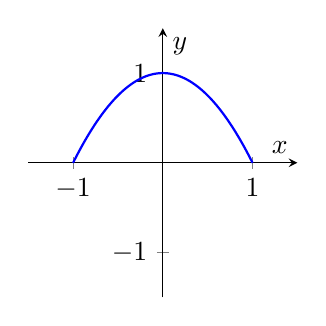
\begin{tikzpicture}
            \begin{axis}[
                xlabel=$x$,
                ylabel=$y$,
                xmin=-1.5,
                xmax=1.5,
                ymin=-1.5,
                ymax=1.5,
                axis lines=middle,
                width=5cm,
                height=5cm,
                samples=90 % número de muestras para la función
            ]
            
            \addplot[blue, thick, domain=-1:1] {(1-x^2)};
            \end{axis}
            \end{tikzpicture}
        \end{figure}
\end{itemize}


\section{Bases ortogonales}
\noindent
Si la base que cogemos del subespacio $U$ es ortogonal, esto es que:
$$\langle \tilde{\varphi_i}, \tilde{\varphi_j} \rangle = 0 ~~\forall i\neq j$$
Entonces, el sistema de ecuaciones se convierte en un sistema diagonal:
$$\langle \tilde{\varphi_k}, \tilde{\varphi_k} \rangle a_k = \langle f, \tilde{\varphi_k} \rangle~~k \in \{0, \ldots, m\}$$
Por lo que:
$$a_k = \dfrac{\langle f, \tilde{\varphi_k} \rangle}{\langle \tilde{\varphi_k}, \tilde{\varphi_k} \rangle}~~k \in \{0, \ldots, m\}$$
Y la mejor aproximación se calcula de la forma:
$$u = \sum_{k=0}^m \dfrac{\langle f, \tilde{\varphi_k} \rangle}{\langle \tilde{\varphi_k}, \tilde{\varphi_k} \rangle}\tilde{\varphi_k}$$

\bigskip
\begin{definicion}[Suma de Fourier]
    A la expresión:
    $$u = \sum_{k=0}^m \dfrac{\langle f, \tilde{\varphi_k} \rangle}{\langle \tilde{\varphi_k}, \tilde{\varphi_k} \rangle}\tilde{\varphi_k}$$
    Se le llama \textbf{$m$-ésima suma de Fourier} de $f$ asociada a la base ortogonal $\{\tilde{\varphi_0}, \tilde{\varphi_1},
        \ldots, \tilde{\varphi_m}\}$.\\

    \noindent
    A la cantidad:
    $$a_k = \dfrac{\langle f, \tilde{\varphi_k} \rangle}{\langle \tilde{\varphi_k}, \tilde{\varphi_k} \rangle}~~~~k \in \{0, \ldots, m\}$$
    Se le llama \textbf{$k$-ésimo coeficiente de Fourier} de $f$ asociado a la base ortongonal $\{\tilde{\varphi_0}, \tilde{\varphi_1},
        \ldots, \tilde{\varphi_m}\}$.\\
\end{definicion}

\subsection{Algoritmo de Gram-Schmidt}
\begin{teo}[Algoritmo de Gram-Schmidt]
    Sea $\{\varphi_0, \varphi_1, \ldots, \varphi_m\}$ una base de $U$, es posible obtener una base ortogonal
    $\{\tilde{\varphi_0}, \tilde{\varphi_1}, \ldots, \tilde{\varphi_m}\}$ de la forma:
    $$\tilde{\varphi_0} = \varphi_0$$
    $$\tilde{\varphi_k} = \varphi_k - \sum_{j=0}^{k-1} \dfrac{\langle \varphi_k, \tilde{\varphi_j} \rangle}
        {\langle \tilde{\varphi_j}, \tilde{\varphi_j} \rangle} \tilde{\varphi_j}~~~~k \in \{1,2, \ldots, m\}$$
    Como consecuencia, sabemos de la existencia de las bases ortogonales.
\end{teo}
\begin{proof}
    Realizamos inducción sobre $k = \dim \cc{L} \{\varphi_0, \varphi_1, \ldots, \varphi_k\}$:
    \begin{itemize}
        \item \underline{Para $k=2$:}

        Sea $\{\varphi_0, \varphi_1\}$ una base de $\cc{L}\{\varphi_0, \varphi_1\}$ con $\dim
        \cc{L}\{\varphi_0, \varphi_1\} = 2$:\par
    Construimos la base:\newline
    $$\tilde{\varphi_0} = \varphi_0$$
    $$\tilde{\varphi_1} = \varphi_1 - \dfrac{\langle \varphi_1, \tilde{\varphi_0} \rangle}
        {\langle \tilde{\varphi_0}, \tilde{\varphi_0} \rangle} \tilde{\varphi_0}$$
    $$\tilde{\varphi_1} \in \cc{L}\{\tilde{\varphi_0}, \varphi_1\} = \cc{L}\{\varphi_0, \varphi_1\}$$

    \noindent
    Comprobemos que $\tilde{\varphi_1}$ es ortogonal a $\tilde{\varphi_0}$ y que son linealmente independientes
    (vamos a demostrar que esto segundo es consecuencia de lo primero):
    $$\langle \tilde{\varphi_1}, \tilde{\varphi_0} \rangle = \langle \varphi_1, \tilde{\varphi_0} \rangle -
        \dfrac{\langle \varphi_1, \tilde{\varphi_0} \rangle}{\langle \tilde{\varphi_0}, \tilde{\varphi_0} \rangle}
        \langle \tilde{\varphi_0}, \tilde{\varphi_0} \rangle = 0 \Rightarrow \tilde{\varphi_1} \perp \tilde{\varphi_0}$$

    Supongamos que son linealmente dependientes: $\exists a,b \in \R \mid a\tilde{\varphi_0} + b \tilde{\varphi_1} = 0$:
    $$0 = \langle a\tilde{\varphi_0} + b\tilde{\varphi_1}, \tilde{\varphi_0} \rangle = a\langle \tilde{\varphi_0},
        \tilde{\varphi_0} \rangle + b \langle \tilde{\varphi_0}, \tilde{\varphi_1} \rangle \mathop{=}^{\tilde{\varphi_0}
        \perp \tilde{\varphi_1}} a\langle \tilde{\varphi_0}, \tilde{\varphi_0} \rangle = 0 \Leftrightarrow a = 0$$
    $$0 = \langle a\tilde{\varphi_0} + b\tilde{\varphi_1}, \tilde{\varphi_1} \rangle = a \langle \tilde{\varphi_0},
        \tilde{\varphi_1} \rangle + b\langle \tilde{\varphi_1}, \tilde{\varphi_1} \rangle \mathop{=}^{\tilde{\varphi_0}
        \perp \tilde{\varphi_1}} b\langle \tilde{\varphi_1}, \tilde{\varphi_1} \rangle = 0 \Leftrightarrow b = 0$$
    Luego $a = b = 0 \Rightarrow$ son linealmente independientes (consecuencia de ser ortogonales).

        \item \underline{Sea cierto para $k-1$:}

        $$\{\tilde{\varphi_0}, \tilde{\varphi_1}, \ldots, \tilde{\varphi}_{k-1}\} \mbox{ es una base de }
        \cc{L}\{\varphi_0, \varphi_1, \ldots, \varphi_{k-1}\} \mbox{ en la que:}$$
    $$\tilde{\varphi_i} \perp \tilde{\varphi_j}~~~~ i \neq j~~ i,j \in \{0, 1, \ldots, k-1\}$$
    Construimos:
    $$\tilde{\varphi_k} = \varphi_k - \sum_{j=0}^{k-1} \dfrac{\langle \varphi_k, \tilde{\varphi_j} \rangle}
        {\langle \tilde{\varphi_j}, \tilde{\varphi_j} \rangle} \tilde{\varphi_j}$$
    Comprobemos que sea ortogonal al resto (y por tanto, linealmente independientes):
    $$\forall j \in \{0, \ldots, k-1\}: \langle \tilde{\varphi_k}, \tilde{\varphi_j} \rangle = \langle \varphi_k,
        \tilde{\varphi_j} \rangle - \sum_{i=0}^{k-1} \dfrac{\langle \tilde{\varphi_k}, \tilde{\varphi_i} \rangle}
        {\langle \tilde{\varphi_i}, \tilde{\varphi_i} \rangle} \langle \tilde{\varphi_i}, \tilde{\varphi_j} \rangle=$$
    $$= \langle \varphi_k, \tilde{\varphi_j} \rangle - \sum_{i=0}^{k-1} \dfrac{\langle \tilde{\varphi_k},
            \tilde{\varphi_i} \rangle} {\langle \tilde{\varphi_i}, \tilde{\varphi_i} \rangle} \delta_{ij} \langle \tilde{\varphi_j},
        \tilde{\varphi_j} \rangle = \langle \varphi_k,
        \tilde{\varphi_j} \rangle - \dfrac{\langle \tilde{\varphi_k}, \tilde{\varphi_j} \rangle}
        {\langle \tilde{\varphi_j}, \tilde{\varphi_j} \rangle} \langle \tilde{\varphi_j}, \tilde{\varphi_j} \rangle = 0$$
    Por lo que $\tilde{\varphi_k} \perp \tilde{\varphi_j}~~~~\forall j \in \{0, \ldots, k-1\} \Rightarrow$ es linealmente
    independiente con todos ellos $\Rightarrow \{\tilde{\varphi_0}, \tilde{\varphi_1}, \ldots, \tilde{\varphi}_{k-1},
        \tilde{\varphi_k}\}$ es una base de $\cc{L}\{\varphi_0, \varphi_1, \ldots, \varphi_{k-1}, \varphi_k\}$.
    \end{itemize}
    
\end{proof}


\begin{ejemplo}
 Dado el siguiente producto escalar dentro de $\bb{P}_2$:
$$\langle f,g \rangle = \int_0^1 f(x)g(x)~dx~~~~\forall f,g \in \bb{P}_2$$
Buscar una base ortogonal a partir de la base $\{1,x,x^2\}$\\

\noindent
Aplicamos el algoritmo de Gram-Schmidt:\par
Dada $\{\varphi_i\} \mid \varphi_i = x^i~~i \in \{0,1,2\}$, construimos $\{\tilde{\varphi_i}\}$ como sigue:
$$\tilde{\varphi_0} = \varphi_0$$
$$\tilde{\varphi_1} = \varphi_1 - \dfrac{\langle \varphi_1, \tilde{\varphi_0} \rangle}{\langle \tilde{\varphi_0},
        \tilde{\varphi_0} \rangle} \tilde{\varphi_0}$$
$$\tilde{\varphi_2} = \varphi_2 - \dfrac{\langle \varphi_2, \tilde{\varphi_0} \rangle}{\langle \tilde{\varphi_0},
        \tilde{\varphi_0} \rangle} \tilde{\varphi_0} - \dfrac{\langle \varphi_2, \tilde{\varphi_1} \rangle}{\langle \tilde{\varphi_1},
        \tilde{\varphi_1} \rangle} \tilde{\varphi_1}$$

Calculamos los respectivos productos escalares:
$$\langle \varphi_1, \tilde{\varphi_0} \rangle = \int_0^1 x~dx = \dfrac{1}{2}
\qquad 
\langle \tilde{\varphi_0}, \tilde{\varphi_0} \rangle = \int_0^1 dx = 1$$
$$\tilde{\varphi_1} = \varphi_1 - \dfrac{\langle \varphi_1, \tilde{\varphi_0} \rangle}{\langle \tilde{\varphi_0},
        \tilde{\varphi_0} \rangle} \tilde{\varphi_0} = x - \dfrac{1}{2} \cdot 1 = x - \dfrac{1}{2}$$
\begin{equation*}
    \langle \varphi_2, \tilde{\varphi_0} \rangle = \int_0^1 x^2~dx = \dfrac{1}{3}
\qquad
\langle \varphi_2, \tilde{\varphi_1} \rangle = \int_0^1 x^2(x - \dfrac{1}{2})~dx = \dfrac{1}{12}
\qquad
\langle \tilde{\varphi_1}, \tilde{\varphi_1} \rangle = \int_0^1 (x-\dfrac{1}{2})^2~dx = \dfrac{1}{12}
\end{equation*}
$$\tilde{\varphi_2} = \varphi_2 - \dfrac{\langle \varphi_2, \tilde{\varphi_0} \rangle}{\langle \tilde{\varphi_0},
        \tilde{\varphi_0} \rangle} \tilde{\varphi_0} - \dfrac{\langle \varphi_2, \tilde{\varphi_1} \rangle}{\langle \tilde{\varphi_1},
        \tilde{\varphi_1} \rangle} \tilde{\varphi_1} = x^2 - \dfrac{1}{3} \cdot 1 - \left(x- \dfrac{1}{2}\right) = x^2 - x + \dfrac{1}{6}$$

\noindent
Por tanto, la base buscada es:
$$\left\{1, x-\dfrac{1}{2}, x^2-x+\dfrac{1}{6}\right\}$$
\end{ejemplo}

\subsection{Bases ortonormales}
\noindent Las bases ortonormales son bases ortogonales en las que la norma de cada elemento de la base es igual a 1.\\

\noindent
A la hora de obtener bases ortonormales podemos hacer dos procedimientos a partir del anterior algoritmo de Gram-Schmidt:
\begin{itemize}
    \item Aplicar el algoritmo de Gram-Schmidt y normalizar la base: esto es, aplicar el algoritmo sobre uan base para
          obtener una base ortogonal y luego escalar los vectores de la base para que tengan norma 1.
    \item O aplicar el algoritmo de Gram-Schmidt modificado, que consiste en obtener un vector de la base de Gram-Schmidt,
          normalizarlo y volver a aplicar el algoritmo con este vector normalizado y repetir sucesivamente.
\end{itemize}

\noindent
En la práctica, suele ser más cómodo hacerlo de la primera forma aunque esto tiene un inconveniente, ya que este
método es inestable numéricamente mientras que el segundo es estable numéricamente. Por tanto, cuando queramos evitar
errores al conseguir una base ortonormal a partir de una base para un subespacio de una dimensión considerable,
es conveniente aplicar el segundo método.\\

\noindent
\textbf{Normalización de vectores.} Dado un vector $v \in V$ que queremos normalizar, esto es $\|v\|=1 \Leftrightarrow \|v\|^2 = 1$.
Escalaremos $v$ de la siguiente forma:
$$\overline{v} = \dfrac{1}{\langle v,v \rangle}v = \dfrac{1}{\sqrt{\|v\|^2}}v = \dfrac{1}{\|v\|}v$$

De esta forma:
$$\|\overline{v}\| = \sqrt{\|\overline{v}\|^2} = \sqrt{\langle \overline{v},\overline{v} \rangle} =
    \sqrt{\left\langle \dfrac{1}{\|v\|}v,\dfrac{1}{\|v\|}v \right\rangle} = \sqrt{\dfrac{\langle v,v \rangle}{\|v\|^2}} =
    \sqrt{\dfrac{\|v\|^2}{\|v\|^2}} = 1$$

\subsection{Utilidad de bases ortogonales}
\noindent
Dado un producto escalar de la forma:
$$\langle x^i, x^j \rangle = \int_0^1 x^{i+j}~dx = \dfrac{1}{i+j+1}$$
Tenemos que la matriz de coeficientes del sistema que nos permite calcular la mejor aproximación respecto de la base
del estilo $\{x^i\}~~i \in \{0, 1, \ldots, n\}$ del subespacio $U=\bb{P}_n$ del espacio vectorial de polinomios es:
$$G=\left(\begin{array}{ccccc}
            \langle 1,1 \rangle   & \langle x,1 \rangle   & \langle x^2,1 \rangle & \ldots & \langle x^n,1 \rangle   \\
            \langle 1,x \rangle   & \langle x,x \rangle   & \ldots                & \ldots & \langle x^n, x \rangle  \\
            \langle 1,x^2 \rangle & \vdots                & \ddots                & \ddots & \vdots                  \\
            \vdots                & \vdots                & \ddots                & \ddots & \vdots                  \\
            \langle 1,x^n \rangle & \langle x,x^n \rangle & \ldots                & \ldots & \langle x^n,x^n \rangle
        \end{array}\right) = \left( \begin{array}{ccccc}
            1            & \dfrac{1}{2}   & \dfrac{1}{3} & \ldots & \dfrac{1}{n}   \\
                         &                &              &                         \\
            \dfrac{1}{2} & \dfrac{1}{3}   & \ldots       & \ldots & \dfrac{1}{n+1} \\
            \dfrac{1}{3} & \vdots         & \ddots       & \ddots & \vdots         \\
            \vdots       & \vdots         & \ddots       & \ddots & \vdots         \\
            \dfrac{1}{n} & \dfrac{1}{n+1} & \ldots       & \ldots & \dfrac{1}{2n}
        \end{array} \right)$$
Llamada matriz de Hilbert, donde todos los elementos de cada antidiagonal son iguales entre sí (matriz de Hankel):
$$\langle x^2,1 \rangle = \langle x,x \rangle = \langle 1,x^2 \rangle = \int_0^1 x^2~dx = \dfrac{1}{3}$$

\noindent
Dicha matriz está muy mal condicionada y para solventar el problema numérico al que nos enfrentamos, se suele aplicar
el algoritmo de Gram-Schmidt sobre la base anterior para obtener una base ortogonal y construir nuestro sistema
con dicha base, formando un sistema diagonal cuya resolución no nos supone ningún problema.\\

\noindent
Este procedimiento puede llegar a ser hasta más eficiente que el trabajar directamente con la matriz de Hilbert para
dimensiones grandes.

\section{Polinomios ortogonales}
\begin{definicion}[Polinomios Ortogonales]
    Dado un producto escalar $\langle \cdot,\cdot \rangle$, una familia de polinomios $\{P_n(x)\}_{n\geq 0}$ se dice que es
    una sucesión de polinomios ortogonales (SPO) si verifica:
    \begin{enumerate}
        \item $grd(P_n) = n$
        \item $\langle P_n, P_m \rangle = 0~~~~\forall n \neq m$
    \end{enumerate}
    \noindent
    Por tanto, tenemos que $\{P_0, P_1, \ldots, P_m\}$ es una base ortogonal de $\bb{P}_m$
\end{definicion}

\noindent
Una sucesión de polinomios ortogonales mónica (SPOM) (es decir, de coeficiente líder 1) puede obtenerse aplicando el algoritmo de
Gram-Schmidt a la base $\{1, x, x^2, \ldots, x^m\}$ de $\bb{P}_m$.

\noindent
Además, las sucesiones de polinomios ortogonales son únicas salvo constante multiplicativa.

\begin{teo}
    Dado un producto escalar $\langle \cdot,\cdot \rangle$ y sea $\{P_n\}_{n \geq 0}$ la correspondiente SPOM, entonces existen
    $\{c_n\}_{n \geq 0}$ y $\{\lambda_n\}_{n\geq 1}$ con $\lambda_n>0$ $\forall n$, tales que:
    $$P_{n+1}(x) = (x-c_{n+1})P_n(x) - \lambda_{n+1}P_{n-1}(x)~~~~\forall n \geq 0$$
    Con $P_{-1}(x) = 0$ y $P_0(x) = 1$\\

    \noindent
    En particular:
    $$c_{n+1} = \dfrac{\langle xP_n(x), P_n(x) \rangle}{\langle P_n(x),P_n(x) \rangle}$$
    $$\lambda_{n+1} = \dfrac{\langle P_n(x), P_n(x) \rangle}{\langle P_{n-1}(x),P_{n-1}(x) \rangle}$$
\end{teo}
\begin{proof}
    Dados los $n+1$ primeros polinomios ortogonales mónicos de una sucesión, nos disponemos a calcular el siguiente:
    $$xP_n(x) \in \bb{P}_{n+1} \Rightarrow xP_n(x) = \sum_{j=1}^{n+1} d_jP_j(x)$$
    $$\langle xP_n, P_k \rangle = \sum_{j=0}^{n+1} d_j \langle P_j, P_k \rangle = \sum_{j=0}^{n+1} d_j \delta_{kj} \langle P_j, P_k \rangle
        = d_k \langle P_k, P_k \rangle$$
    Luego:
    $$d_k = \dfrac{\langle xP_n, P_k \rangle}{\langle P_k, P_k \rangle} = \dfrac{\langle P_n, xP_k \rangle}
        {\langle P_k, P_k \rangle} = 0 \Leftrightarrow k+1<n \Leftrightarrow k<n-1$$
    Por lo que:
    $$d_j = 0~~~~\forall j \in \{0, 1, \ldots, n-2\}$$
    De donde concluimos:
    $$xP_n(x) = \sum_{j=1}^{n+1} d_jP_j(x) = \sum_{j=n-1}^{n+1} d_jP_j(x) =$$
    $$=d_{n-1}P_{n-1}(x) + d_nP_n(x) + d_{n+1}P_{n+1}(x)$$

    \noindent
    $xP_n(x)$ es de grado $n+1$ y su coeficiente líder es 1 por ser mónico, en el término de la derecha, el único
    monomio de grado $n+1$ es el de $d_{n+1}P_{n+1}(x)$ que es $d_{n+1}$, por lo que concluimos que $d_{n+1}=1$
    $$xP_n(x)=d_{n-1}P_{n-1}(x) + d_nP_n(x) + P_{n+1}(x)$$
    $$P_{n+1}(x) = (x-d_n)P_n(x) - d_{n-1}P_{n-1}(x)$$
    Y tenemos que:
    $$c_{n+1}=d_n~~~~~~\lambda_{n+1}=d_{n-1}$$
\end{proof}

\bigskip
\noindent
A continuación, la siguiente parte de los apuntes no es relevante en lo que se refiere a la asignatura de
Métodos Numéricos I, el lector puede leerlo para su disfrute.

\subsection{Polinomios de Jacobi}
\noindent
Se obtienen como la familia de polinomios ortogonales asociados a la función de peso dada por:
$$w(x) = (1-x)^\alpha(1+x)^\beta~~~~x \in [-1,1]~~\alpha, \beta > -1$$
Denotamos por $P_n^{(\alpha, \beta)}(x)$ a los polinomios de Jacobi, que verifican la condición de normalización:
$$P_n^{(\alpha, \beta)}(1) = \binom{n+\alpha}{n}$$

\noindent
Estos presentan como casos particulaes a las familias de polinomios de:
\begin{itemize}
    \item Chebyshev de primera especie, con $\alpha = \beta = \dfrac{-1}{2}$.
    \item Chebyshev de segunda espacie, con $\alpha = \beta = \dfrac{1}{2}$.
    \item Legendre, con $\alpha = \beta = 0$.
    \item Gegenbauer o ultraesféricos, con $\alpha = \beta$.
\end{itemize}

\noindent
Todos ellos de coeficiente líder:
$$P_n^{(\alpha, \beta)}(x) = \dfrac{(n + \alpha + \beta + 1)}{2n!}x^n + \ldots$$

\noindent
\textbf{Fórmula de Rodrigues.}
$$P_n^{(\alpha, \beta)}(x) = \dfrac{(-1)^n}{2^nn!}(1-x)^{-\alpha}(1+x)^{-\beta}D^n((1-x)^{n+\alpha}(1+x)^{n+\beta})~~\alpha, \beta>$$

\noindent
\textbf{Ortogonalidad.}
$$\int_{-1}^1 P_n^{(\alpha,\beta)}(x) P_m^{(\alpha, \beta)}(x) (1-x)^\alpha(1+x)^\beta~dx = \left\{ \begin{array}{ll}
        \tau_n \delta_{mn} & n=m      \\
        0                  & n \neq m
    \end{array} \right.$$
$$\tau_n = \dfrac{2^{\alpha + \beta + 1}}{2n + \alpha + \beta + 1} \dfrac{\Gamma(n+ \alpha + 1) \Gamma(n+\beta + 1)}
    {\Gamma(n+\alpha + \beta + 1)n!}$$

\noindent
\textbf{Fórmula de recurrencia.}
$$xP_n^{(\alpha, \beta)}(x) = \dfrac{2(n+1)(n+\alpha + \beta + 1)}{(2n + \alpha + \beta +1)(2n + \alpha + \beta + 2)}P_{n+1}^{(\alpha,\beta)}(x) + $$
$$+ \dfrac{\beta^2-\alpha^2}{(2n+\alpha+\beta)(2n+\alpha+\beta+2)}P_n^{(\alpha + \beta)}(x) + $$
$$+ \dfrac{2(n+\alpha)(n+\beta)}{(2n+\alpha+\beta)(2n+\alpha+\beta+1)}P_{n-1}^{(\alpha,\beta)}(x)$$

\subsection{Polinomios de Lagrere}
\noindent
Se obtienen como la familia de polinomio ortogonales asociados a la función peso dada por:
$$w(x) = x^\alpha e^{-x}~~~~x \in [0,+\infty[~~\alpha >1$$
Los correspondientes momentos existen y verifican:
$$\int_0^{+\infty}x^nx^\alpha e^{-x}~dx = \int_0^{+\infty}x^{n+\alpha}e^{-x}~dx = \Gamma(n+\alpha)$$
Notemos por $\{L_n^{(\alpha)}(x)\}_{n\geq 0}$ a los polinomios de Laguerre con coeficiente líder $L_n^{(\alpha)} =
    \dfrac{(-1)^n}{n!}x^n + \ldots$

\noindent
\textbf{Fórmula de Rodrigues.}
$$L_n^{(\alpha)}(x) = \dfrac{1}{n!}x^{\alpha}e^{-x}D^n(x^{n+\alpha e^{-x}})~~~~\alpha >-1$$

\noindent
\textbf{Ortogonalidad.}
$$\int_0^{+\infty}L_m^{(\alpha)}(x) L_n^{(\alpha)}(x) x^\alpha e^{-x}~dx = \left\{ \begin{array}{ll}
        \dfrac{\Gamma(n + \alpha + 1)}{n!}\gamma_{mn} & n = m    \\
        0                                             & n \neq m
    \end{array} \right.$$

\noindent
\textbf{Relación de recurrencia.}
$$(n+1)L_{n+1}^{(\alpha)}(x) = (2n + \alpha + 1 - x)L_n^{(\alpha)}(x) - (n+\alpha)L_{n-1}^{(\alpha)}(x)$$

\subsection{Polinomios de Hermite}
\noindent
Se obtienen como la familia de polinomios ortogonales a la función peso dada por:
$$w(x) = e^{-x^2}~~~~\forall x \in \R$$
$\todon$, notaremos por $H_n(x)$ al polinomio ortogonal con respecto a $w(x)$ y cuyo coeficiente líder es $H_n(x) = 2^nx^n + \ldots$.\\

\noindent
\textbf{Fórmula de Rodrigues.}
$$H_n(x) = (-1)^n e^{x^2} D^n(e^{-x^2})$$

\noindent
\textbf{Ortogonalidad.}
$$\int_{-\infty}^{+\infty}H_m(x) H_n(x) e^{-x^2}~dx = \left\{ \begin{array}{ll}
        2^n n! \sqrt{\pi}\delta_{nm} & n = m    \\
        0                            & n \neq m
    \end{array} \right.$$

\noindent
\textbf{Relación de recurrencia.}
$$H_n(x) = 2xH_{n-1}(x) -2nH_{n-2}(x)$$


\section{Ejercicios}
Los ejercicios relativos a este tema están disponbles en la sección \ref{sec:Rel4}.